\documentclass[11pt]{article}  % 11 points is a good size
\usepackage{fullpage}
\usepackage{pdfpages}
\usepackage{graphicx}
\usepackage{hyperref}    
\begin{document}
\title{Assignment 1}
\author{Benjamin Sorenson}
\maketitle                     % generates the title

\section{Written Questions}
    \begin{enumerate}
    \item \lbrack20 points\rbrack Performance measures for an agent could be
    designed based on the effects the agent has on the environment or
    according to the behaviors of the agent. Explain briefly what is the difference,
    provide an example for each, and explain if one of the two choices is best
    and why.
    \paragraph{Answer:}
    Taking two examples from the book, in the case of the vacuum cleaner agent,
    one could define a performance measure by the amount of dirt cleaned up in a
    single 8 hour shift, awarding more points for more dirt cleaned---a
    performance measure according to the behaviours of the agent.
    Alternatively, one could define a performance measure by awarding one point
    for each clean square at each time step---a performance measure according
    to the effects the agent has on the environment.
    \par
    In the case of a performance measure designed according to the behaviours of
    the agent, we reward behavior that we think will lead to the desired effects
    on the environment rather than reward for the desired effects directly.
    This can allow a rational agent to maximize its performance measure without
    the desired effects to the environment. For example, as the book points out,
    a rational vacuum cleaner agent that is maximizing the amount of dirt
    cleaned in an 8 hour period could maximize its performance measure by
    cleaning up the dirt, dumping it back on the floor and cleaning it again. 
    For this reason, it is better to define a performance
    measure based on the desired effects to the environment rather than the
    behaviors of the agent.
    \item \lbrack30 points\rbrack You are given the following problem: Given a
    5-gallon jug filled with water and an empty 2-gallon jug how can you have
    precisely 1 gallon of water in the 2-gallon jug? Assume you can fill the
    jugs with water as many times as desired, but you cannot measure how much
    water is in each jug. When you move water out of a jug you can either fill
    up the other jug or dump the water.
    \par 
    You are to formulate the problem using a state-space search
    representation.
    \par 
    Describe (precisely):
    \begin{enumerate}
      \item what is the initial state
      \par
      The initial state is a 5-gallon jug (referred to as ``5G'' for the
      remained or the description) filled with water and an empty 2-gallon jug
      (referred to as ``2G'' for the remainder of the description).  Note: for
      the remainder of this description a state will be denoted as \(\lbrace
      Jug1 : NumberofGallons, Jug2 : NumberofGallons\rbrace\).  For example, the
      initial state wwould be \(\lbrace 5G:5, 2G:0\rbrace\). 
      \item the goal test
      \par
      Precisely 1 gallon of water in the 2G.
      \item the actions (called in the textbook successor function)
      \begin{enumerate}
        \item \texttt{pour\_into(PouringJug, ReceivingJug)} \par
        \emph{Definition}: if the amount of water in \texttt{PouringJug}
        (\(g1\)) plus the amount of water in \texttt{ReceivingJug} (\(g2\)) is
        \(\le\) to the capacity of \texttt{ReceivingJug} (\(G2\)), the amount of
        water in \texttt{ReceivingJug} is set to \(g1 + g2\), otherwise,  fill
        \texttt{RecievingJug} to \(G2\) and set the level of \texttt{PouringJug}
        to \(g1 + g2 - G2\)
        \par 
        Example: \[RESULT(\lbrace 5G : 5, 2G:0\rbrace, pour\_into(5G,
        2G)) = \lbrace 5G : 3, 2G:2\rbrace\]
        \item \texttt{empty(Jug)}
        \par\emph{Definition}: set the level of \texttt{Jug} to \(0\)
        \par
        Example: \[RESULT(\lbrace 5G : 5, 2G : 0\rbrace, empty(5G)) = \lbrace
        5G:0, 2G : 0 \rbrace\]
        \item \texttt{fill(Jug)}
        \par\emph{Definition}: set the level of \texttt{Jug} to its maximum
        capacity
        \par
        Example: \[RESULT(\lbrace 5G : 5, 2G : 0\rbrace, fill(2G)) = \lbrace
        5G:5, 2G : 2 \rbrace\]
      \end{enumerate}
      \item the path cost
      \par
      Each step costs 1 so the path cost is the number of steps in the path
      \item the state-space for the problem
      \par
      The state-space is any state of fullness of the two-gallon and
      five-gallon jugs reachable by the actions \texttt{pour\_into(Jug1, Jug2)},
      \texttt{fill(Jug)}, and \texttt{empty(Jug)} performed on the initial state
      and any resultant states.  Though other states are possible, any state can
      be trivially converted to one of the states reachable by the initial state
      in this problem definition in at most two actions.
      \item is the state-space a tree or a graph?
      \par
      The sate space is a graph since there are repeated states.
      \item what search algorithm would you use and why?
      \par 
      I would use a uniform-cost search because the search space is small, and
      it will always find an optimal solution.
      \item show graphically the search space explored and the solution (there
      might be more than one solution)
      \par
      Next two pages show 
        \begin{enumerate}
          \item The search space explored
          \item The optimal soluion
        \end{enumerate}
    The color of the arrows indicate the action according to the following
    legend
    \par\center{
    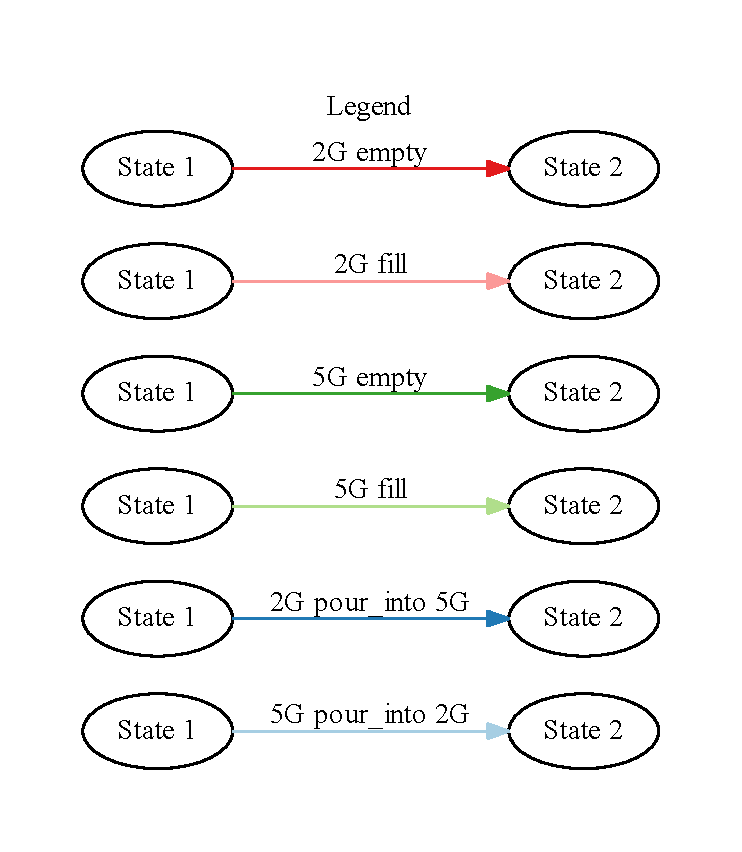
\includegraphics[scale=.75]{Legend.pdf}
    }
    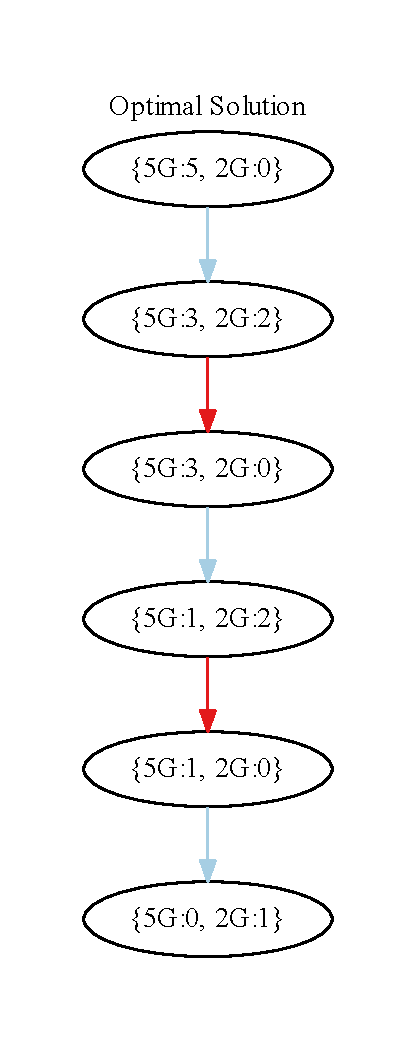
\includepdf{my_graph_optimal.pdf}
    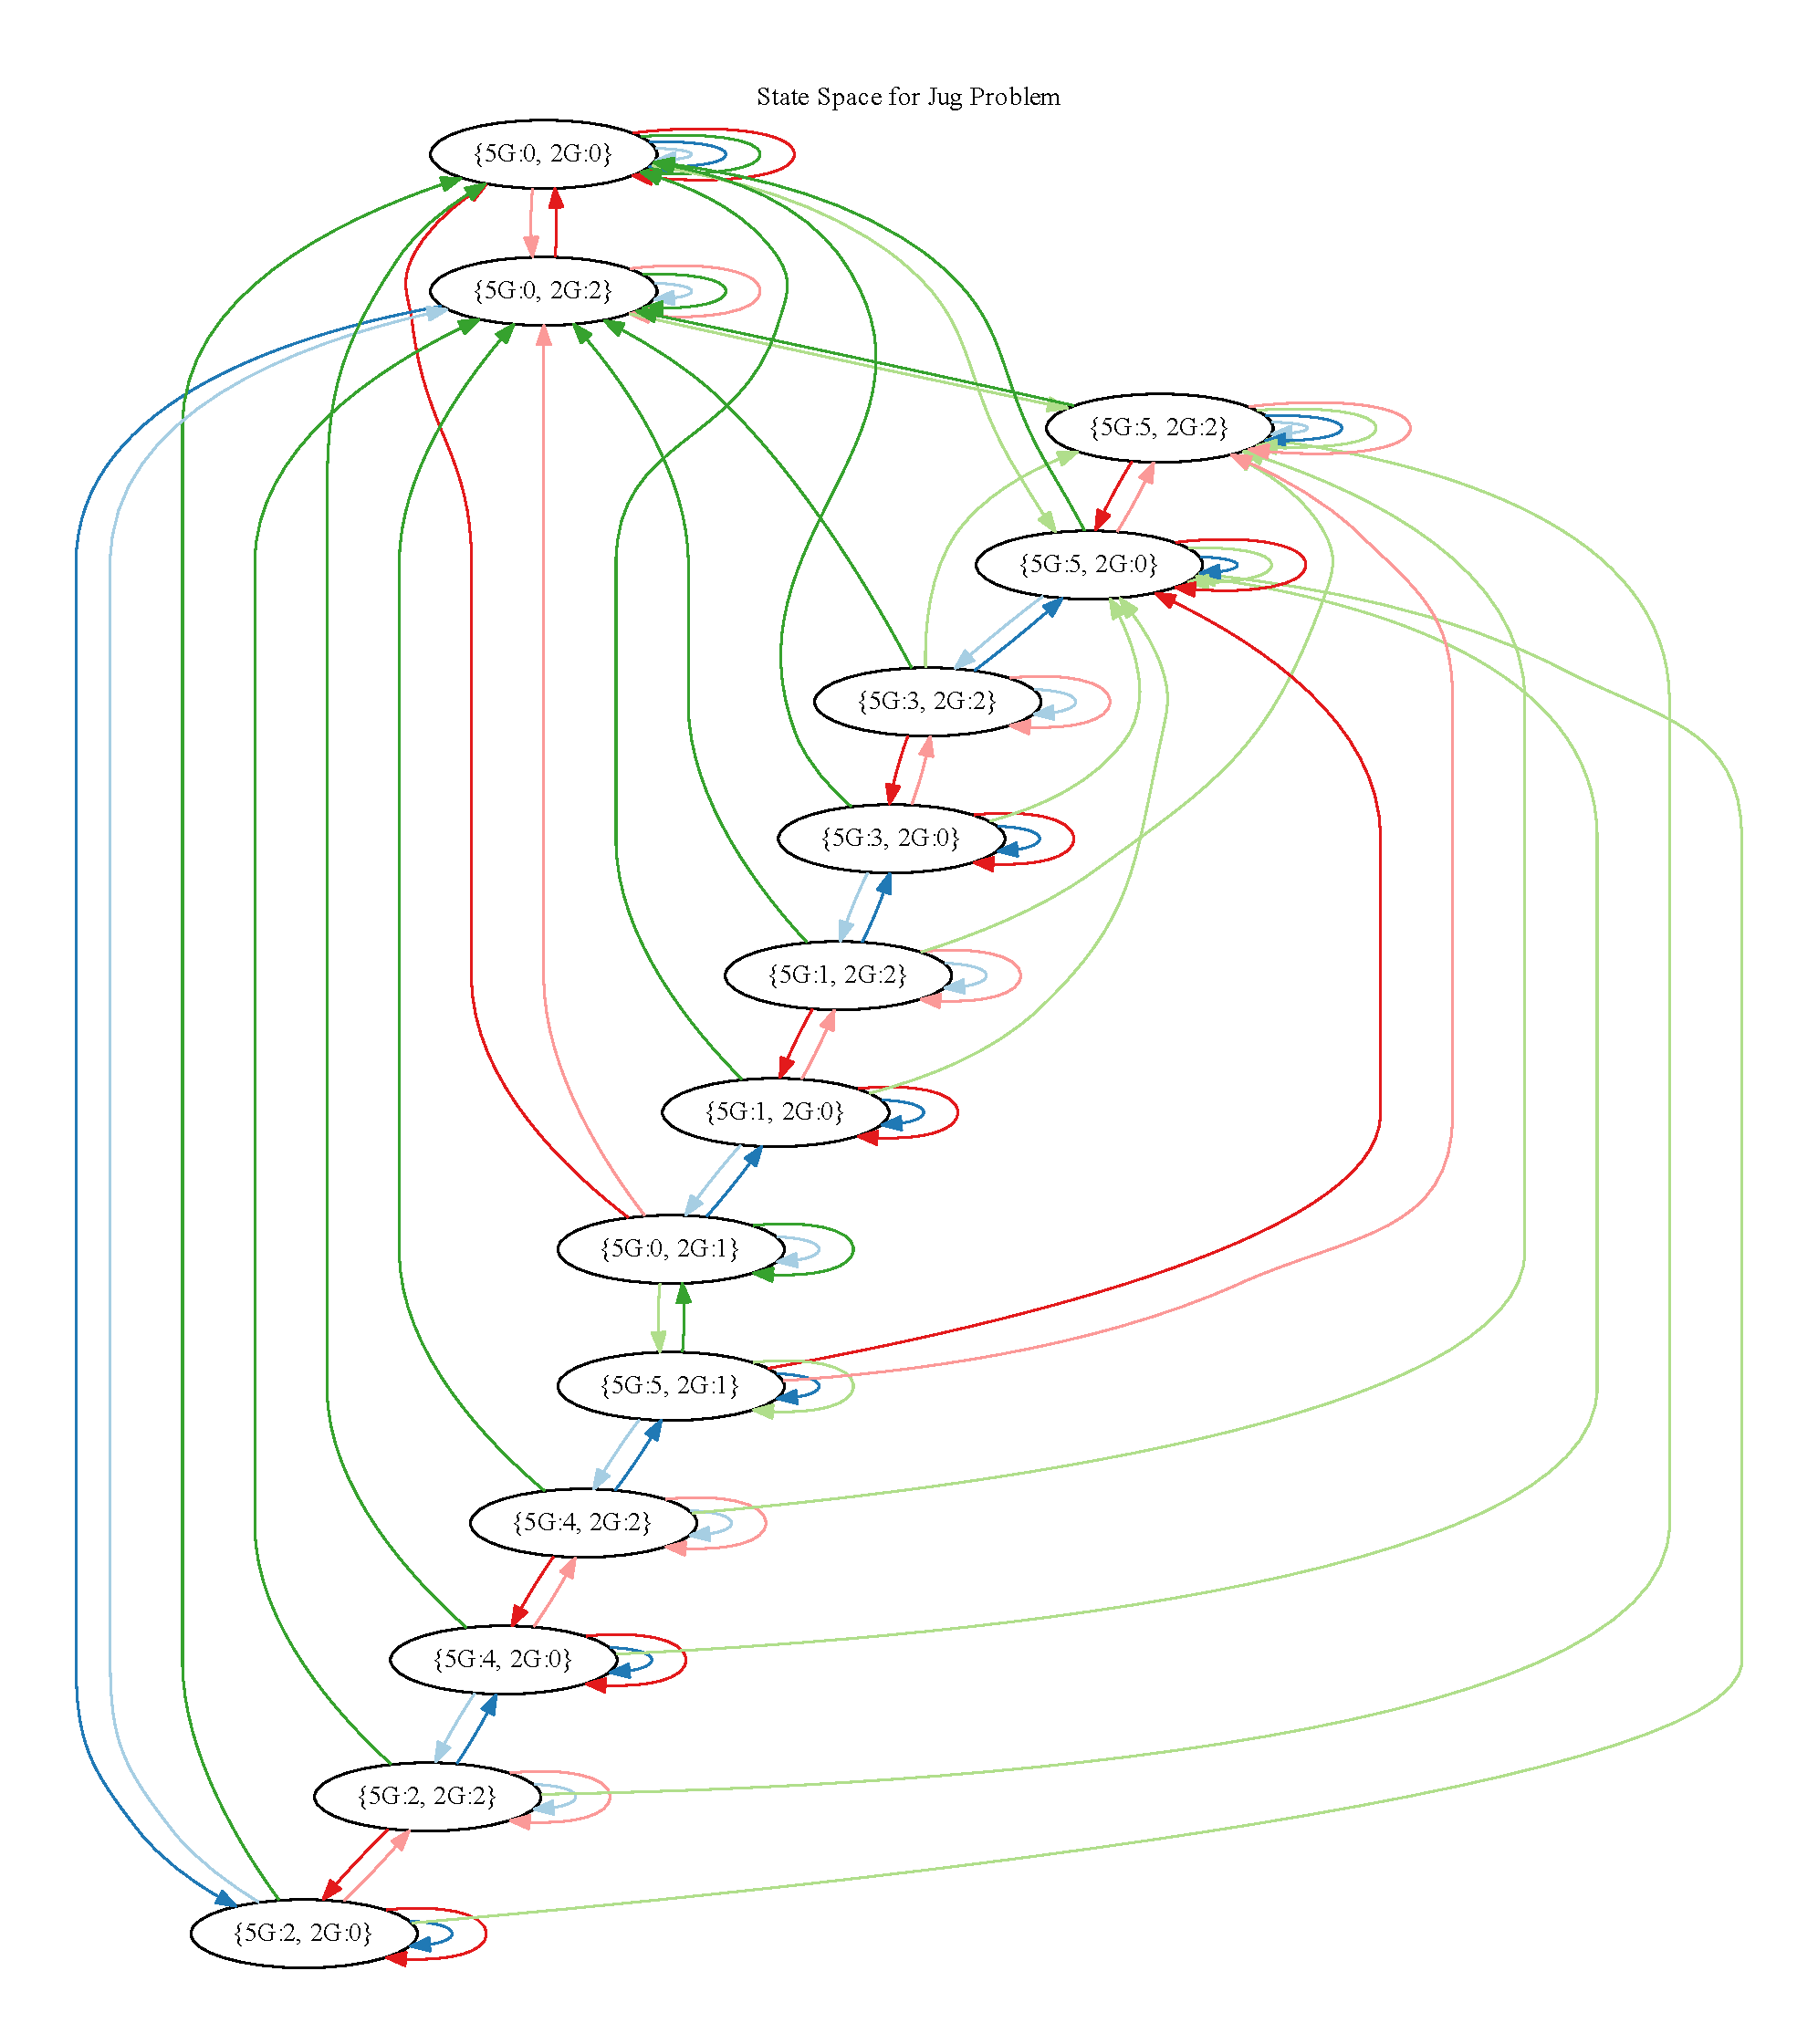
\includepdf{my_graph_pruned.pdf}
    \end{enumerate}
    \item \lbrack20 points\rbrack There has been a lot of discussion recently
    in the news and on the web on the dangers of AI, started by Stephen Hawking and Elon
    Musk
    \par.
    \begin{enumerate}
    \item Search for a few on line writings on the controversy and summarize (in
    1/2 to 1 page) the main arguments made.
    \item Read the white paper by Eric Horvitz outlining the project
    \href{https://stanford.app.box.com/s/266hrhww2l3gjoy9euar}{One Hundred Year Study on Artificial Intelligence}.
    Can you think of some additional topics not listed there? or could you add more
    questions to one of the topics listed? Summarize your thoughts (in a few
    paragraphs).
    \par
    \subsection{Ethics}
    I wish I could spend more time thinking about the topics covered.  In each
    topic, the central concern seems to be to one degree or another ``What are
    the consequences of turning over traditionally human decisions over to
    machines?'' and, in the other direction ``What can we
    accomplish (for good for bad) with the aid intelligent machines?'' 
    Personally, I'm most looking forward to autonomous assistants that don't
    take any direction---they observe your behaviour and try to help out.  For
    the first few weeks or months, they may do almost nothing, and suddenly
    rudimentary tasks begin to get completed on their own.  Of course, this
    comes with its own set of ethical concerns.  What if you're a serial killer,
    and you now have a serial killer assisstant---even if checks are put in
    place so that the machine can't assist killing or some other hard safe-guard, 
    real life is fuzzy.  Where doee the threshold lie between contributing to 
    nefarious activity and not?  Who decides?   

    \subsection{Educations}    
    I saw an info-graphic (I can't remember where, now), that put education near
    the bottom of fields most likely impacted by ``Data Science.''  I
    tend to instead agree with the idea that education is one of the key areas
    of opportunity for AI.  I've heard (source?) that the most difficult part of
    teaching is figuring out what when wrong when a student comes up with an incorrect
    solution---this difficulty is then multiplied by the number of students that
    a teacher has to observe.  A machince that could perfectly and
    objectively observed, memorize, and perform rigorous analyses to assist a
    teacher in discovering these paths leading to incorrect understanding of
    the material, I would have to beleive, would be invaluable to both teachers
    and students.  Maybe this would take the form of a study tool where not only
    is the student shown the correct answer when, but also given instruction
    specific to the deficiency in their understanding of the material.
    
   
    
    \subsection{Augmentation}
    
    The first concern is addressed most directly in law and ethics.  Who is
    responsible when a machine makes the ``wrong'' decision? Is it the
    programmer, the owner? Will we see a new standard of right and wrong as
    rigorous analysis and unbiased memory picks informs our actions? 
    \par
    With regard to economics, we're already seeing impacts of smart, targeted
    advertising.  There's the famous story of Target figuring out a teenage girl
    was pregnant before her parents.  I don'tk 
    \end{enumerate}
    \end{enumerate}
\end{document}